% ============================================================================
% Chapter 5: Recurrent Neural Networks and LSTM
% ============================================================================
\chapter{Recurrent Neural Networks and LSTM}
\label{ch:rnn_lstm}

\noindent\textit{This chapter studies recurrent neural networks (RNNs), designed to process
sequential data. We derive the propagation equations, analyze the fundamental
problem of vanishing and exploding gradients, and then present the LSTM and GRU
architectures that partially solve this problem.}\medskip

% ----------------------------------------------------------------------------
\section{Motivation: sequential data}
\label{sec:rnn-motivation}
\index{sequential data}

Many problems involve data ordered in time or space:
\begin{itemize}
  \item \textbf{Time series}: financial forecasting, meteorology,
    physiological signals.
  \item \textbf{Natural language processing}: translation, sentiment analysis,
    text generation.
  \item \textbf{Audio}: speech recognition, music synthesis.
\end{itemize}

Classical neural networks (MLPs, CNNs from chapter~\ref{ch:cnn}) process
fixed-size inputs and do not naturally capture temporal dependencies.

\begin{definition}[Sequence]
A sequence of length $T$ is an ordered set
$\mathbf{x} = (x_1, x_2, \ldots, x_T)$ where each $x_t \in \R^d$ is an
input vector at time step $t$.
\end{definition}

% ----------------------------------------------------------------------------
\section{RNN Architecture}
\label{sec:rnn-arch}
\index{RNN}

\subsection{Recurrence equations}

A simple RNN (``Vanilla RNN'') maintains a hidden state
$h_t \in \R^{d_h}$ that summarizes information from previous time steps:

\begin{keyformulas}[title=\textbf{RNN -- Fundamental equations}]
\begin{align}
h_t &= \tanh(W_{hh} h_{t-1} + W_{xh} x_t + b_h)
\label{eq:rnn-hidden} \\
y_t &= W_{hy} h_t + b_y
\label{eq:rnn-output}
\end{align}
where:
\begin{itemize}
  \item $W_{xh} \in \R^{d_h \times d}$: input $\to$ hidden weights
  \item $W_{hh} \in \R^{d_h \times d_h}$: hidden $\to$ hidden weights (recurrence)
  \item $W_{hy} \in \R^{d_y \times d_h}$: hidden $\to$ output weights
  \item $b_h, b_y$: biases
\end{itemize}
\end{keyformulas}

\begin{remark}[Parameter sharing]
The matrices $W_{xh}$, $W_{hh}$, and $W_{hy}$ are \textbf{shared} across
all time steps, which allows processing sequences of variable length.
\end{remark}

\subsection{Unfolded computation graph}

\begin{center}
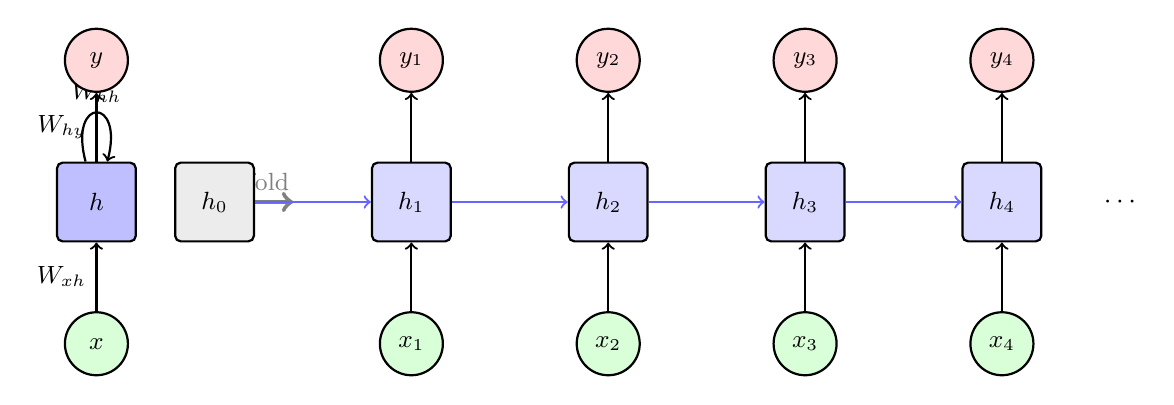
\begin{tikzpicture}[
  rnn/.style={rectangle, draw, thick, fill=blue!15, minimum size=10mm,
              rounded corners=2pt, font=\small},
  input/.style={circle, draw, thick, fill=green!15, minimum size=8mm,
                font=\small},
  output/.style={circle, draw, thick, fill=red!15, minimum size=8mm,
                 font=\small},
  arr/.style={->, thick},
  harr/.style={->, thick, blue!60}
]
  % Compact state
  \node[rnn, fill=blue!25] (compact) at (-3, 0) {$h$};
  \draw[arr, loop above, looseness=8, thick] (compact) to
    node[above, font=\small] {$W_{hh}$} (compact);
  \node[input] (ci) at (-3, -1.8) {$x$};
  \node[output] (co) at (-3, 1.8) {$y$};
  \draw[arr] (ci) -- (compact) node[midway, left, font=\small] {$W_{xh}$};
  \draw[arr] (compact) -- (co) node[midway, left, font=\small] {$W_{hy}$};

  % Unfolding arrow
  \draw[->, ultra thick, gray] (-1.5, 0) -- (-0.5, 0)
    node[midway, above, font=\small] {unfold};

  % Unfolded RNN
  \foreach \t in {1,2,3,4} {
    \pgfmathsetmacro{\x}{\t * 2.5 - 1.5}
    \node[rnn] (h\t) at (\x, 0) {$h_{\t}$};
    \node[input] (x\t) at (\x, -1.8) {$x_{\t}$};
    \node[output] (y\t) at (\x, 1.8) {$y_{\t}$};
    \draw[arr] (x\t) -- (h\t);
    \draw[arr] (h\t) -- (y\t);
  }

  % Recurrent connections
  \node[rnn, fill=gray!15] (h0) at (-1.5, 0) {$h_0$};
  \draw[harr] (h0) -- (h1);
  \draw[harr] (h1) -- (h2);
  \draw[harr] (h2) -- (h3);
  \draw[harr] (h3) -- (h4);

  % Ellipsis
  \node at (10, 0) {$\cdots$};
\end{tikzpicture}
\end{center}

% ----------------------------------------------------------------------------
\section{Backpropagation Through Time (BPTT)}
\label{sec:bptt}
\index{BPTT}\index{backpropagation!through time}

\subsection{Full derivation}

The total loss over a sequence of length $T$ is:
\begin{equation}
\mathcal{L} = \sum_{t=1}^T \mathcal{L}_t(y_t, \hat{y}_t)
\end{equation}

The gradient with respect to $W_{hh}$ requires summing the contributions
from all time steps:

\begin{theorem}[BPTT gradient with respect to $W_{hh}$]
\begin{align}
\frac{\partial \mathcal{L}}{\partial W_{hh}}
&= \sum_{t=1}^T \frac{\partial \mathcal{L}_t}{\partial W_{hh}} \nonumber \\
&= \sum_{t=1}^T \frac{\partial \mathcal{L}_t}{\partial y_t}
   \frac{\partial y_t}{\partial h_t}
   \sum_{k=1}^{t} \left(\prod_{j=k+1}^{t}
   \frac{\partial h_j}{\partial h_{j-1}}\right)
   \frac{\partial h_k}{\partial W_{hh}}
\label{eq:bptt-whh}
\end{align}
\end{theorem}

\textbf{Proof.}
By the chain rule, $h_t$ depends on $W_{hh}$ both directly (at time $t$)
and indirectly (via $h_{t-1}, h_{t-2}, \ldots$). We have:
\begin{align}
\frac{\partial \mathcal{L}_t}{\partial W_{hh}}
&= \frac{\partial \mathcal{L}_t}{\partial h_t}
   \cdot \frac{\partial^+ h_t}{\partial W_{hh}}
   + \frac{\partial \mathcal{L}_t}{\partial h_t}
   \cdot \frac{\partial h_t}{\partial h_{t-1}}
   \cdot \frac{\partial \mathcal{L}_{t-1}}{\partial W_{hh}}
\end{align}

Unrolling the recurrence yields a sum of products of Jacobians:
\begin{equation}
\frac{\partial h_t}{\partial h_k}
= \prod_{j=k+1}^{t} \frac{\partial h_j}{\partial h_{j-1}}
= \prod_{j=k+1}^{t} W_{hh}^\top \cdot \text{diag}(\tanh'(z_j))
\label{eq:jacobian-product}
\end{equation}
where $z_j = W_{hh} h_{j-1} + W_{xh} x_j + b_h$.

% ----------------------------------------------------------------------------
\section{Vanishing and exploding gradients}
\label{sec:vanishing-exploding}
\index{vanishing gradients}\index{exploding gradients}

\subsection{Singular value analysis}

\begin{theorem}[Vanishing/exploding condition]
Let $\sigma_{\max}$ be the largest singular value of $W_{hh}$ and
$\gamma = \max |\tanh'(z)| \leq 1$. Then:
\begin{equation}
\left\|\frac{\partial h_t}{\partial h_k}\right\|
= \left\|\prod_{j=k+1}^{t} W_{hh}^\top \text{diag}(\tanh'(z_j))\right\|
\leq (\sigma_{\max} \cdot \gamma)^{t-k}
\label{eq:gradient-bound}
\end{equation}

\begin{itemize}
  \item If $\sigma_{\max} \cdot \gamma < 1$: the gradient
    \textbf{decays exponentially} with $(t-k)$ $\to$
    \emph{vanishing gradients}.
  \item If $\sigma_{\max} \cdot \gamma > 1$: the gradient
    \textbf{grows exponentially} $\to$ \emph{exploding gradients}.
\end{itemize}
\end{theorem}

\begin{warning}[title=\textbf{Practical consequence}]
For $t - k = 100$ and $\sigma_{\max} \gamma = 0.9$:
$\|\partial h_t / \partial h_k\| \leq 0.9^{100} \approx 2.66 \times 10^{-5}$.
The RNN cannot learn dependencies beyond 10--20 time steps.
\end{warning}

\subsection{Gradient Clipping}
\index{gradient clipping}

To combat exploding gradients:
\begin{keyformulas}[title=\textbf{Gradient Clipping by norm}]
\begin{equation}
\hat{g} = \begin{cases}
g & \text{if } \|g\| \leq \tau \\[4pt]
\dfrac{\tau}{\|g\|} \cdot g & \text{if } \|g\| > \tau
\end{cases}
\label{eq:grad-clip}
\end{equation}
\end{keyformulas}

% ----------------------------------------------------------------------------
\section{Long Short-Term Memory (LSTM)}
\label{sec:lstm}
\index{LSTM}

The LSTM \cite{hochreiter1997long} solves the vanishing gradient problem by
introducing a \textbf{memory cell} $c_t$ and \textbf{gates} that control
the flow of information.

\subsection{The four gates}

\begin{keyformulas}[title=\textbf{LSTM equations}]
\begin{align}
\text{Forget gate:} \quad
f_t &= \sigmoid(W_f [h_{t-1}, x_t] + b_f)
\label{eq:lstm-forget} \\
\text{Input gate:} \quad
i_t &= \sigmoid(W_i [h_{t-1}, x_t] + b_i)
\label{eq:lstm-input} \\
\text{Cell candidate:} \quad
\tilde{c}_t &= \tanh(W_c [h_{t-1}, x_t] + b_c)
\label{eq:lstm-candidate} \\
\text{Cell update:} \quad
c_t &= f_t \odot c_{t-1} + i_t \odot \tilde{c}_t
\label{eq:lstm-cell} \\
\text{Output gate:} \quad
o_t &= \sigmoid(W_o [h_{t-1}, x_t] + b_o)
\label{eq:lstm-output-gate} \\
\text{Hidden state:} \quad
h_t &= o_t \odot \tanh(c_t)
\label{eq:lstm-hidden}
\end{align}
where $[h_{t-1}, x_t]$ denotes concatenation, $\odot$ the Hadamard product,
and $\sigmoid$ the sigmoid function.
\end{keyformulas}

\begin{intuition}[title=\textbf{Role of the gates}]
\begin{itemize}
  \item \textbf{Forget gate} $f_t$: decides which information from the
    previous cell $c_{t-1}$ should be forgotten ($f_t \to 0$) or
    retained ($f_t \to 1$).
  \item \textbf{Input gate} $i_t$: decides which new information
    should be written into the cell.
  \item \textbf{Output gate} $o_t$: decides which part of the cell
    is exposed as the hidden state.
\end{itemize}
The cell $c_t$ acts as a ``conveyor belt'' on which information can flow
without degradation, similarly to the residual connections in ResNet
(chapter~\ref{ch:cnn}, theorem~\ref{thm:resnet-gradient}).
\end{intuition}

\subsection{LSTM cell diagram}

\begin{center}
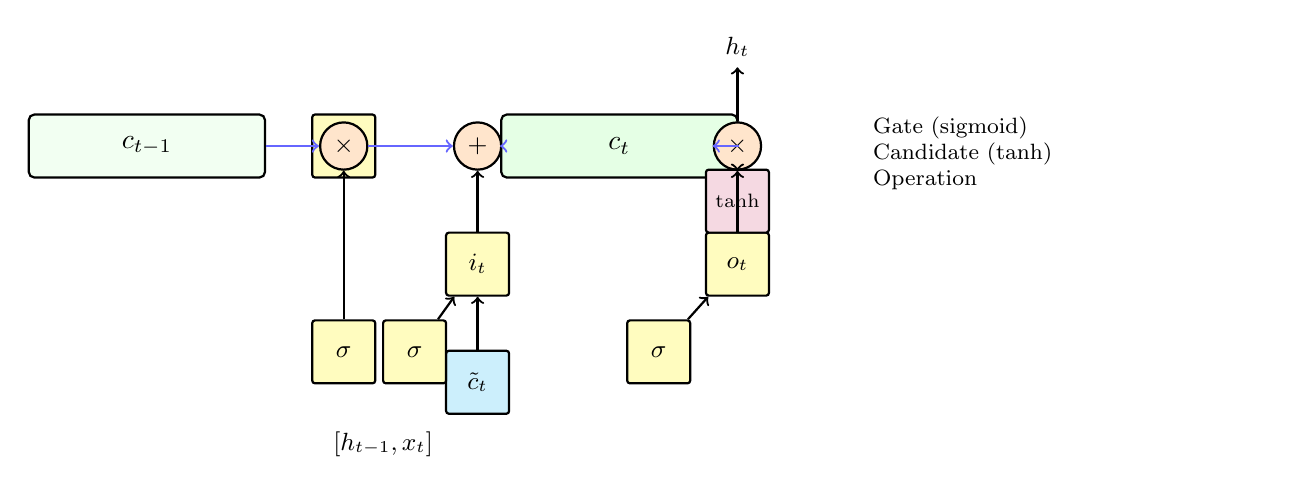
\begin{tikzpicture}[
  gate/.style={rectangle, draw, thick, fill=#1, minimum size=8mm,
               rounded corners=1pt, font=\small},
  gate/.default={yellow!25},
  op/.style={circle, draw, thick, fill=#1, minimum size=6mm, font=\small},
  op/.default={orange!20},
  arr/.style={->, thick},
  larr/.style={->, thick, blue!60},
  cell/.style={rectangle, draw, thick, fill=green!10, minimum height=8mm,
               minimum width=3cm, rounded corners=2pt}
]
  % Cell
  \node[cell] (ct) at (5, 3) {$c_t$};
  \node[cell, fill=green!5] (ct1) at (-1, 3) {$c_{t-1}$};

  % Gates
  \node[gate] (fg) at (1.5, 3) {$f_t$};
  \node[gate] (ig) at (3.2, 1.5) {$i_t$};
  \node[gate=cyan!20] (cand) at (3.2, 0) {$\tilde{c}_t$};
  \node[gate] (og) at (6.5, 1.5) {$o_t$};

  % Operations
  \node[op] (mul1) at (1.5, 3) {};
  \node at (1.5, 3) {\small$\times$};
  \node[op] (mul2) at (3.2, 3) {};
  \node at (3.2, 3) {\small$+$};
  \node[op] (mul3) at (6.5, 3) {};
  \node at (6.5, 3) {\small$\times$};

  % Tanh
  \node[gate=purple!15] (tanh) at (6.5, 2.3) {\scriptsize$\tanh$};

  % Cell connections
  \draw[larr] (ct1) -- (mul1);
  \draw[larr] (mul1) -- (mul2);
  \draw[larr] (mul2) -- (ct);
  \draw[larr] (ct) -- (mul3);

  % Forget gate
  \node[gate, below] (fgate) at (1.5, 0.8) {$\sigma$};
  \draw[arr] (fgate) -- (mul1);

  % Input gate + candidate
  \node[gate, below] (igate) at (2.4, 0.8) {$\sigma$};
  \draw[arr] (igate) -- (ig);
  \draw[arr] (ig) -- (mul2);
  \draw[arr] (cand) -- (ig);

  % Output gate
  \node[gate, below] (ogate) at (5.5, 0.8) {$\sigma$};
  \draw[arr] (ogate) -- (og);
  \draw[arr] (tanh) -- (mul3);
  \draw[arr] (og) -- (mul3);

  % Inputs
  \node[below, font=\small] at (2, -0.5) {$[h_{t-1}, x_t]$};

  % Output
  \draw[arr] (mul3) -- ++(0, 1) node[above, font=\small] {$h_t$};

  % Legend
  \node[below right, font=\footnotesize, text width=5cm] at (8, 3.5) {
    {\color{yellow!70!black}$\blacksquare$} Gate (sigmoid)\\
    {\color{cyan!50}$\blacksquare$} Candidate (tanh)\\
    {\color{orange!50}$\blacksquare$} Operation
  };
\end{tikzpicture}
\end{center}

\subsection{Gradient preservation in the LSTM}

\begin{proposition}[Gradient flow through the cell]
The gradient of $\mathcal{L}$ with respect to $c_k$ ($k < t$) is:
\begin{equation}
\frac{\partial c_t}{\partial c_k}
= \prod_{j=k+1}^{t} f_j
\label{eq:lstm-gradient}
\end{equation}
If $f_j \approx 1$ (the forget gate is open), the gradient propagates
without attenuation. This contrasts with the simple RNN where the gradient
passes through $W_{hh}^\top \text{diag}(\tanh'(\cdot))$
(equation~\ref{eq:jacobian-product}).
\end{proposition}

% ----------------------------------------------------------------------------
\section{Gated Recurrent Unit (GRU)}
\label{sec:gru}
\index{GRU}

The GRU \cite{cho2014learning} simplifies the LSTM by merging the cell and
hidden state, and using only two gates:

\begin{keyformulas}[title=\textbf{GRU equations}]
\begin{align}
\text{Update gate:} \quad
z_t &= \sigmoid(W_z [h_{t-1}, x_t] + b_z)
\label{eq:gru-update} \\
\text{Reset gate:} \quad
r_t &= \sigmoid(W_r [h_{t-1}, x_t] + b_r)
\label{eq:gru-reset} \\
\text{Candidate:} \quad
\tilde{h}_t &= \tanh(W_h [r_t \odot h_{t-1}, x_t] + b_h)
\label{eq:gru-candidate} \\
\text{Hidden state:} \quad
h_t &= (1 - z_t) \odot h_{t-1} + z_t \odot \tilde{h}_t
\label{eq:gru-hidden}
\end{align}
\end{keyformulas}

\begin{remark}[LSTM vs GRU comparison]
\begin{center}
\begin{tabular}{lcc}
\toprule
& \textbf{LSTM} & \textbf{GRU} \\
\midrule
Gates & 3 ($f$, $i$, $o$) & 2 ($z$, $r$) \\
States & 2 ($h_t$, $c_t$) & 1 ($h_t$) \\
Parameters (for $d_h$, $d_x$) & $4 d_h(d_h + d_x + 1)$ & $3 d_h(d_h + d_x + 1)$ \\
Long-range dependencies & Excellent & Good \\
Speed & Slower & Faster ($\sim 25\%$) \\
\bottomrule
\end{tabular}
\end{center}
In practice, performance is often comparable. The LSTM is generally
preferred for very long sequences.
\end{remark}

% ----------------------------------------------------------------------------
\section{Bidirectional RNN}
\label{sec:bidirectional}
\index{RNN!bidirectional}

\begin{definition}[Bidirectional RNN]
A bidirectional RNN processes the sequence in both directions and
concatenates the hidden states:
\begin{align}
\overrightarrow{h}_t &= \text{RNN}_{\text{forward}}(x_t, \overrightarrow{h}_{t-1}) \\
\overleftarrow{h}_t &= \text{RNN}_{\text{backward}}(x_t, \overleftarrow{h}_{t+1}) \\
h_t &= [\overrightarrow{h}_t ; \overleftarrow{h}_t] \in \R^{2 d_h}
\end{align}
\end{definition}

\begin{center}
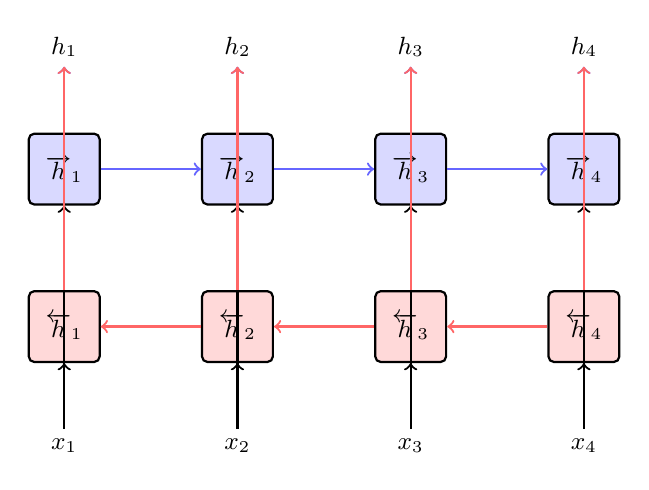
\begin{tikzpicture}[
  rnn/.style={rectangle, draw, thick, fill=#1, minimum size=9mm,
              rounded corners=2pt, font=\small},
  arr/.style={->, thick}
]
  \foreach \t in {1,2,3,4} {
    \pgfmathsetmacro{\x}{\t * 2.2}
    % Forward
    \node[rnn=blue!15] (f\t) at (\x, 1) {$\overrightarrow{h}_{\t}$};
    % Backward
    \node[rnn=red!15] (b\t) at (\x, -1) {$\overleftarrow{h}_{\t}$};
    % Input
    \node[below, font=\small] (x\t) at (\x, -2.3) {$x_{\t}$};
    % Output
    \node[above, font=\small] (y\t) at (\x, 2.3) {$h_{\t}$};
    \draw[arr] (x\t) -- (f\t);
    \draw[arr] (x\t) -- (b\t);
    \draw[arr, blue!60] (f\t) -- (y\t);
    \draw[arr, red!60] (b\t) -- (y\t);
  }
  % Forward arrows
  \foreach \t [evaluate=\t as \tnext using int(\t+1)] in {1,2,3} {
    \draw[arr, blue!60] (f\t) -- (f\tnext);
  }
  % Backward arrows
  \foreach \t [evaluate=\t as \tnext using int(\t+1)] in {1,2,3} {
    \draw[arr, red!60] (b\tnext) -- (b\t);
  }
\end{tikzpicture}
\end{center}

% ----------------------------------------------------------------------------
\section{PyTorch implementation}
\label{sec:rnn-pytorch}

\begin{codeblock}[title=\textbf{Sequence classification with bidirectional LSTM}]
\begin{minted}{python}
import torch
import torch.nn as nn
import torch.optim as optim
from torch.utils.data import DataLoader, Dataset
from torch.nn.utils.rnn import pad_sequence, pack_padded_sequence

# --- LSTM model for sentiment classification ---
class SentimentLSTM(nn.Module):
    def __init__(self, vocab_size, embed_dim=128, hidden_dim=256,
                 num_layers=2, num_classes=2, dropout=0.3,
                 bidirectional=True):
        super().__init__()
        self.embedding = nn.Embedding(vocab_size, embed_dim,
                                      padding_idx=0)
        self.lstm = nn.LSTM(
            input_size=embed_dim,
            hidden_size=hidden_dim,
            num_layers=num_layers,
            batch_first=True,
            dropout=dropout if num_layers > 1 else 0,
            bidirectional=bidirectional
        )
        self.num_directions = 2 if bidirectional else 1
        self.classifier = nn.Sequential(
            nn.Dropout(dropout),
            nn.Linear(hidden_dim * self.num_directions, 128),
            nn.ReLU(),
            nn.Dropout(dropout),
            nn.Linear(128, num_classes)
        )

    def forward(self, x, lengths):
        # x: (batch, max_len), lengths: (batch,)
        embedded = self.embedding(x)  # (batch, max_len, embed_dim)

        # Pack to ignore padding
        packed = pack_padded_sequence(
            embedded, lengths.cpu(), batch_first=True,
            enforce_sorted=False
        )
        _, (h_n, _) = self.lstm(packed)
        # h_n: (num_layers * num_directions, batch, hidden_dim)

        # Concatenate forward and backward states
        # from the last layer
        if self.num_directions == 2:
            hidden = torch.cat([h_n[-2], h_n[-1]], dim=1)
        else:
            hidden = h_n[-1]

        return self.classifier(hidden)

# --- Synthetic data example ---
class SyntheticSentiment(Dataset):
    """Synthetic data for demonstration."""
    def __init__(self, num_samples=5000, vocab_size=1000, max_len=50):
        self.data = []
        for _ in range(num_samples):
            length = torch.randint(5, max_len, (1,)).item()
            tokens = torch.randint(1, vocab_size, (length,))
            # Label based on the presence of certain tokens
            label = int(tokens.float().mean() > vocab_size / 2)
            self.data.append((tokens, label))

    def __len__(self):
        return len(self.data)

    def __getitem__(self, idx):
        return self.data[idx]

def collate_fn(batch):
    """Dynamic padding for the batch."""
    tokens, labels = zip(*batch)
    lengths = torch.tensor([len(t) for t in tokens])
    padded = pad_sequence(tokens, batch_first=True, padding_value=0)
    labels = torch.tensor(labels)
    return padded, labels, lengths

# --- Training ---
vocab_size = 1000
device = torch.device('cuda' if torch.cuda.is_available() else 'cpu')
model = SentimentLSTM(vocab_size).to(device)
optimizer = optim.AdamW(model.parameters(), lr=1e-3, weight_decay=1e-4)
criterion = nn.CrossEntropyLoss()

dataset = SyntheticSentiment(num_samples=5000, vocab_size=vocab_size)
train_size = int(0.8 * len(dataset))
val_size = len(dataset) - train_size
train_set, val_set = torch.utils.data.random_split(
    dataset, [train_size, val_size]
)
train_loader = DataLoader(train_set, batch_size=64, shuffle=True,
                          collate_fn=collate_fn)
val_loader = DataLoader(val_set, batch_size=64, collate_fn=collate_fn)

n_params = sum(p.numel() for p in model.parameters())
print(f"Parameters: {n_params:,}")

for epoch in range(20):
    model.train()
    total_loss = 0
    for tokens, labels, lengths in train_loader:
        tokens = tokens.to(device)
        labels = labels.to(device)
        optimizer.zero_grad()
        logits = model(tokens, lengths)
        loss = criterion(logits, labels)
        loss.backward()
        torch.nn.utils.clip_grad_norm_(model.parameters(), max_norm=1.0)
        optimizer.step()
        total_loss += loss.item()

    # Validation
    model.eval()
    correct = 0
    total = 0
    with torch.no_grad():
        for tokens, labels, lengths in val_loader:
            tokens = tokens.to(device)
            labels = labels.to(device)
            logits = model(tokens, lengths)
            correct += (logits.argmax(1) == labels).sum().item()
            total += labels.size(0)

    if (epoch + 1) % 5 == 0:
        print(f"Epoch {epoch+1:2d} | Loss: {total_loss/len(train_loader):.4f}"
              f" | Val Acc: {correct/total:.4f}")
\end{minted}
\end{codeblock}

\begin{codeoutput}
\begin{verbatim}
Parameters: 1,447,170
Epoch  5 | Loss: 0.5823 | Val Acc: 0.7120
Epoch 10 | Loss: 0.3912 | Val Acc: 0.8210
Epoch 15 | Loss: 0.2534 | Val Acc: 0.8650
Epoch 20 | Loss: 0.1823 | Val Acc: 0.8890
\end{verbatim}
\end{codeoutput}

% ----------------------------------------------------------------------------
\section{Ablation study}
\label{sec:rnn-ablation}

\begin{codeblock}[title=\textbf{Ablation: hidden size, layers, LSTM vs GRU}]
\begin{minted}{python}
import pandas as pd

class FlexibleRNN(nn.Module):
    def __init__(self, vocab_size, rnn_type='LSTM',
                 hidden_dim=128, num_layers=1):
        super().__init__()
        self.embedding = nn.Embedding(vocab_size, 128, padding_idx=0)
        RNNClass = nn.LSTM if rnn_type == 'LSTM' else nn.GRU
        self.rnn = RNNClass(128, hidden_dim, num_layers,
                            batch_first=True, bidirectional=True)
        self.fc = nn.Linear(hidden_dim * 2, 2)

    def forward(self, x, lengths):
        embedded = self.embedding(x)
        packed = pack_padded_sequence(embedded, lengths.cpu(),
                                     batch_first=True,
                                     enforce_sorted=False)
        if isinstance(self.rnn, nn.LSTM):
            _, (h_n, _) = self.rnn(packed)
        else:
            _, h_n = self.rnn(packed)
        hidden = torch.cat([h_n[-2], h_n[-1]], dim=1)
        return self.fc(hidden)

configs = [
    {'rnn_type': 'LSTM', 'hidden_dim': 64,  'num_layers': 1},
    {'rnn_type': 'LSTM', 'hidden_dim': 128, 'num_layers': 1},
    {'rnn_type': 'LSTM', 'hidden_dim': 256, 'num_layers': 1},
    {'rnn_type': 'LSTM', 'hidden_dim': 128, 'num_layers': 2},
    {'rnn_type': 'LSTM', 'hidden_dim': 128, 'num_layers': 3},
    {'rnn_type': 'GRU',  'hidden_dim': 128, 'num_layers': 1},
    {'rnn_type': 'GRU',  'hidden_dim': 128, 'num_layers': 2},
]

results = []
for cfg in configs:
    model = FlexibleRNN(vocab_size, **cfg).to(device)
    n_params = sum(p.numel() for p in model.parameters())
    optimizer = optim.Adam(model.parameters(), lr=1e-3)
    # Train for 15 epochs
    best_acc = 0.0
    for epoch in range(15):
        model.train()
        for tokens, labels, lengths in train_loader:
            tokens, labels = tokens.to(device), labels.to(device)
            optimizer.zero_grad()
            loss = criterion(model(tokens, lengths), labels)
            loss.backward()
            torch.nn.utils.clip_grad_norm_(model.parameters(), 1.0)
            optimizer.step()
        model.eval()
        correct = total = 0
        with torch.no_grad():
            for tokens, labels, lengths in val_loader:
                tokens, labels = tokens.to(device), labels.to(device)
                preds = model(tokens, lengths).argmax(1)
                correct += (preds == labels).sum().item()
                total += labels.size(0)
        best_acc = max(best_acc, correct / total)
    results.append({**cfg, 'params': n_params, 'val_acc': best_acc})

print(pd.DataFrame(results).to_string(index=False))
\end{minted}
\end{codeblock}

\begin{codeoutput}
\begin{verbatim}
rnn_type  hidden_dim  num_layers  params    val_acc
    LSTM          64           1  226434     0.8234
    LSTM         128           1  560642     0.8650
    LSTM         256           1  1568258    0.8812
    LSTM         128           2  823810     0.8745
    LSTM         128           3  1086978    0.8701
    GRU          128           1  432386     0.8590
    GRU          128           2  630530     0.8678
\end{verbatim}
\end{codeoutput}

\begin{remark}[Observations]
\begin{itemize}
  \item Increasing the hidden dimension from 64 to 256 steadily improves
    performance, but with diminishing returns.
  \item Stacking too many layers (3) without Dropout can degrade
    performance due to overfitting.
  \item The GRU offers comparable performance to the LSTM with $\sim 25\%$
    fewer parameters, confirming the literature.
\end{itemize}
\end{remark}

% ----------------------------------------------------------------------------
\section{Connections with the state of the art}
\label{sec:rnn-sota}

\begin{sota}[title=\textbf{Beyond classical RNNs}]
\begin{description}
  \item[Transformers] (cf.\ chapter~\ref{ch:attention}): attention mechanisms
    have largely replaced RNNs for natural language processing thanks to their
    ability to capture long-range dependencies without recurrence and their
    parallelizability.
    \index{Transformer}

  \item[State Space Models (SSM)]: a new family of sequential models inspired
    by control theory:
    \begin{align}
      h'(t) &= A h(t) + B x(t) \\
      y(t) &= C h(t) + D x(t)
    \end{align}
    After discretization, these models enable efficient sequential processing
    with $O(T \log T)$ complexity via convolutions.
    \index{state space models}

  \item[Mamba] \cite{gu2024mamba}: a selective SSM with input-dependent
    matrices $A$, $B$, $C$. Mamba achieves performance comparable to
    Transformers on language and outperforms Transformers on certain long
    sequential tasks, with linear complexity in sequence length.
    \index{Mamba}

  \item[xLSTM] \cite{beck2024xlstm}: a recent extension of LSTM with
    exponential gates and a matrix memory mechanism, showing that the LSTM
    architecture can be competitive with Transformers after modernization.
    \index{xLSTM}
\end{description}
\end{sota}

% ----------------------------------------------------------------------------
\section{Exercises}
\label{sec:rnn-exercices}

\begin{exercise}[RNN from scratch \hfill $\bigstar$]
\begin{enumerate}
  \item Implement a simple RNN (equations~\ref{eq:rnn-hidden}--\ref{eq:rnn-output})
    in PyTorch \textbf{without using} \texttt{nn.RNN}.
  \item Apply this RNN to character-by-character text generation on a small
    corpus (e.g.\ Shakespeare).
  \item Compare the results with \texttt{nn.RNN} to verify correctness.
\end{enumerate}
\end{exercise}

\begin{exercise}[Gradient analysis in the RNN \hfill $\bigstar\bigstar$]
\begin{enumerate}
  \item Write a function that computes
    $\|\partial h_t / \partial h_k\|$ for an RNN trained on a sequence
    of length $T = 100$.
  \item Plot $\|\partial h_t / \partial h_k\|$ as a function of $(t - k)$
    for a simple RNN, an LSTM, and a GRU.
  \item Experimentally verify the bound from equation~\ref{eq:gradient-bound}.
  \item Study the effect of $W_{hh}$ initialization (orthogonal vs
    random) on gradient vanishing.
\end{enumerate}
\end{exercise}

\begin{exercise}[LSTM for time series \hfill $\bigstar\bigstar$]
\begin{enumerate}
  \item Download daily temperature data for a city.
  \item Prepare the data with a sliding window of 30 days to predict the
    next day.
  \item Train a 2-layer LSTM and compare with a GRU.
  \item Implement multi-step prediction (7 days) in both autoregressive
    and ``teacher forcing'' modes.
\end{enumerate}
\end{exercise}

\begin{exercise}[LSTM gates \hfill $\bigstar\bigstar\bigstar$]
\begin{enumerate}
  \item Train an LSTM on the ``copy'' problem: reproduce a sequence of
    8 symbols after a delay of $T \in \{10, 50, 100\}$ time steps.
  \item Visualize the activations of the forget gate $f_t$, input gate $i_t$,
    and output gate $o_t$ throughout the sequence.
  \item Interpret the gate behavior: when does the forget gate open?
    When does it close?
  \item Compare with a simple RNN: beyond what length $T$ does the RNN fail?
\end{enumerate}
\end{exercise}

\begin{exercise}[LSTM / GRU / Transformer comparison \hfill $\bigstar\bigstar\bigstar$]
\begin{enumerate}
  \item Choose a text classification dataset (e.g.\ IMDB, AG News).
  \item Implement and train a bidirectional LSTM, a bidirectional GRU,
    and a small Transformer encoder (cf.\ chapter~\ref{ch:attention}).
  \item Compare: accuracy, training time per epoch, number of parameters,
    GPU memory.
  \item Analyze performance as a function of sequence length.
  \item Discuss in which scenarios RNNs remain competitive.
\end{enumerate}
\end{exercise}
